\chapter{Sistemas de Información Geográfica}
\label{chap3}
\ifpdf
    \graphicspath{{Chapter3/Chapter3Figs/PNG/}{Chapter3/Chapter3Figs/PDF/}{Chapter3/Chapter3Figs/}}
\else
    \graphicspath{{Chapter3/Chapter3Figs/EPS/}{Chapter3/Chapter3Figs/}}
\fi

\markboth{\hfill \thechapter. Sistemas de Información Geográfica}{\hfill \thechapter. Sistemas de Información Geográfica}

Los SIG o GIS han sido definidos por varios especialistas y estudiosos, sin embargo difieren en ciertos términos. De acuerdo con \citet{Burrough1986PrinciplesAssessment} un SIG es “un conjunto de herramientas para recopilar, almacenar, recuperar a voluntad, transformar y visualizar datos espaciales del mundo real para un conjunto particular de propósitos”. \citet{NCGIA1990IntroductionGIS} lo define como “un sistema de hardware, software y procedimientos diseñado para realizar la captura, almacenamiento, manipulación, análisis, modelización y presentación de datos referenciados espacialmente para la resolución de problemas complejos de planificación y gestión”.

El SIG es una herramienta que favorece el análisis de la información espacial, es por ello que existen miles de trabajos que lo han utilizado y aprovechado. Por ejemplo, \citet{OsorioDominguez2018AnalisisParaguay} realizaron un análisis multitemporal de la pérdida del hábitat y distribución espacial del mono capuchino (sapajus cay) en la ecorregión selva central, Paraguay. \citet{Cabral2018EstrategiasAsuncion} plantearon una estrategia de planificación que contribuya al mejoramiento del manejo integrado de los RSU con servicios diferenciales mediante tecnología SIG aplicada a la cuenca del Arroyo Ferreira en Asunción. \citet{Acosta2006LevantamientoCaballero} realizaron un levantamiento topográfico y SIG para el abastecimiento de energía eléctrica por vía subterránea línea de 220 kV: tramo Estación Puerto Botánico a Parque Caballero.

Ya que el número de terminologías entorno a estos sistemas es muy grande, en este capítulo se explicarán los conceptos básicos que servirán de apoyo para una clara interpretación de los siguientes capítulos donde han sido aplicados.

\section{Origen de los datos espaciales}

Hoy en día, las informaciones que son recolectadas en censos, encuestas o sistemas informáticos van acompañadas de coordenadas de ubicación. Estas informaciones pueden provenir de dispositivos especializados, teléfonos móviles, tabletas o cámaras. En otras ocasiones, pueden ser generadas de forma manual a través de operaciones o dibujándolas directamente en sistemas SIG, CAD (\textit{Computer-Aided Design}) u otros sistemas capacitados para ello.

Resulta muy común, en la actualidad, que dispositivos electrónicos tengan incorporado internamente un receptor GPS. El Sistema de Posicionamiento Global (GPS, \textit{Global Positioning System}) es un sistema que permite determinar la posición de un objeto en la Tierra. Así también, existen otros mecanismos de geolocalización como por ejemplo: las redes inalámbricas, bluetooth, identificación por radiofrecuencia (RFID, \textit{Radio Frequency Identification}), entre otros (Ver Figura \ref{fig:interioresTech}).

\begin{figure}[H]
    \centering
    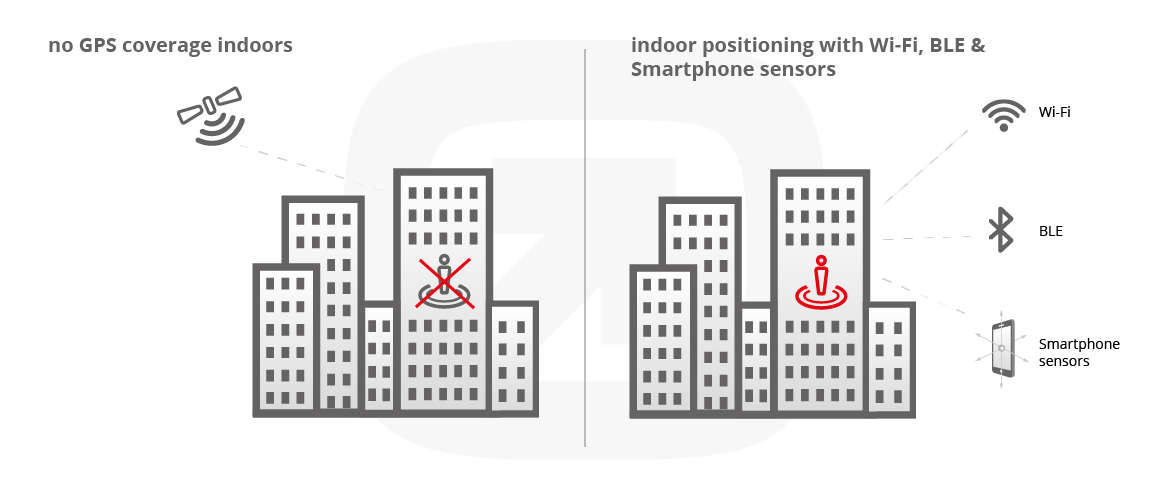
\includegraphics[width=14.5cm]{Indoor_tech.jpg}
    \caption{Tecnologías para localización en interiores. [Fuente: infsoft.com]}
    \label{fig:interioresTech}
\end{figure}

Otra fuente principal de extracción de datos geográficos provienen de las imágenes orto-rectificadas. Las imágenes orto-rectificadas son el resultado del tratamiento de un conjunto de fotografías tanto de satélite como aéreas, donde son corregidas para representar una proyección ortogonal sin efectos de perspectiva, y en la que, por lo tanto, es posible realizar mediciones exactas. Esta fuente es una de las más utilizadas para generar nuevos datos geográficos.

Toda la información en un SIG está vinculada a una referencia espacial, podemos hablar entonces de dos tipos de informaciones: 
\begin{itemize}
    \item \textbf{La información de ubicación:} 
    Describe la posición de las características geográficas particulares en la superficie de la Tierra.
    \item \textbf{La información de atributos:} 
    Describe propiedades de las características geográficas representadas, como su nombre o número, información cuantitativa como su área o longitud, y cualquier otra información asociada a la entidad.
\end{itemize}

Para presentar los datos espaciales, la forma más común es a través de un mapa. Según la Asociación Cartográfica Internacional, un mapa ``es una representación, normalmente a escala y en un medio plano, de una selección de características materiales o abstractas en, o en relación con, la superficie de la Tierra". La escala de un mapa indica la relación de distancia sobre el mapa y su distancia correspondiente sobre la superficie terrestre en la realidad.

La Figura \ref{fig:capasGis} muestra como en los SIG los mapas están organizados lógicamente en un conjunto de capas o temas de información. Un mapa base puede organizarse en capas tales como: carreteras, suelos, límites de estados, ciudades.

\begin{figure}[H]
    \centering
    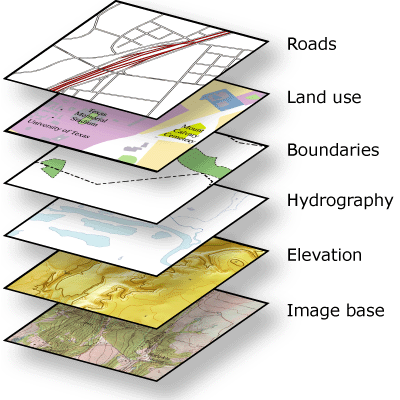
\includegraphics[width=7cm]{capas_gis.png}
    \caption{Organización de capas. [Fuente: arcgis.com]}
    \label{fig:capasGis}
\end{figure}

\section{Referencia espacial}

Los investigadores han confirmado que la superficie de la Tierra no es esférica ni plana sino que es oblata elipsoidal, lo que significa que todos los puntos de la superficie terrestre no son equidistantes del centro geométrico. Para localizar y poder representar los elementos existentes sobre la Tierra en un SIG, existe la necesidad de contar con sistemas de referencia de coordenadas (SRC, en inglés CRS; \textit{Coordinate Reference System}). Los Datums definen los sistemas de referencia que describen el tamaño y la forma de la Tierra, y el origen y la orientación de los sistemas de coordenadas utilizados para mapear la Tierra.

Los tipos de Datums se clasifican en:
\begin{itemize}
    \item \textbf{Horizontal:} 
    Datums que definen la relación entre la Tierra y las coordenadas horizontales. En otras palabras, describe un punto sobre la superficie terrestre, como la latitud y la longitud.
    \item \textbf{Vertical:} 
    Datums que definen superficies de nivel, midiendo elevaciones o profundidades. Algunos se basan en mediciones del nivel del mar y redes de nivelación, otros en mediciones de la gravedad.
    \item \textbf{Completo:} 
    Datums que describen los sistemas verticales y horizontales. Algunos, como el \textit{World Geodetic System 1984} (WGS84), también describen otros parámetros, como la velocidad de rotación de la Tierra y diversas constantes físicas, como la velocidad angular y la constante gravitacional de la Tierra.
\end{itemize}

Por otro lado, los sistemas de referencia espacial se agrupan por lo general en tres categorías: Sistemas de coordenadas geográficas, Sistemas de coordenadas rectangulares (también denominados como: proyectados, planos o cartesianos) y Sistemas no coordinados; los cuáles los detallaremos a continuación.

\subsection{Sistema de coordenadas geográficas}
Los sistemas de coordenadas geográficas se componen de la latitud y la longitud. Las líneas de longitud (también conocidas como meridianos) comienzan en un polo y se propagan hacia afuera hasta que convergen en el polo opuesto. Las líneas de latitud (también conocidas como paralelos) se encuentran en ángulo recto a las líneas de longitud y corren paralelas entre sí (Ver Figura \ref{fig:latitudLongitud}). 

\begin{figure}[H]
    \centering
    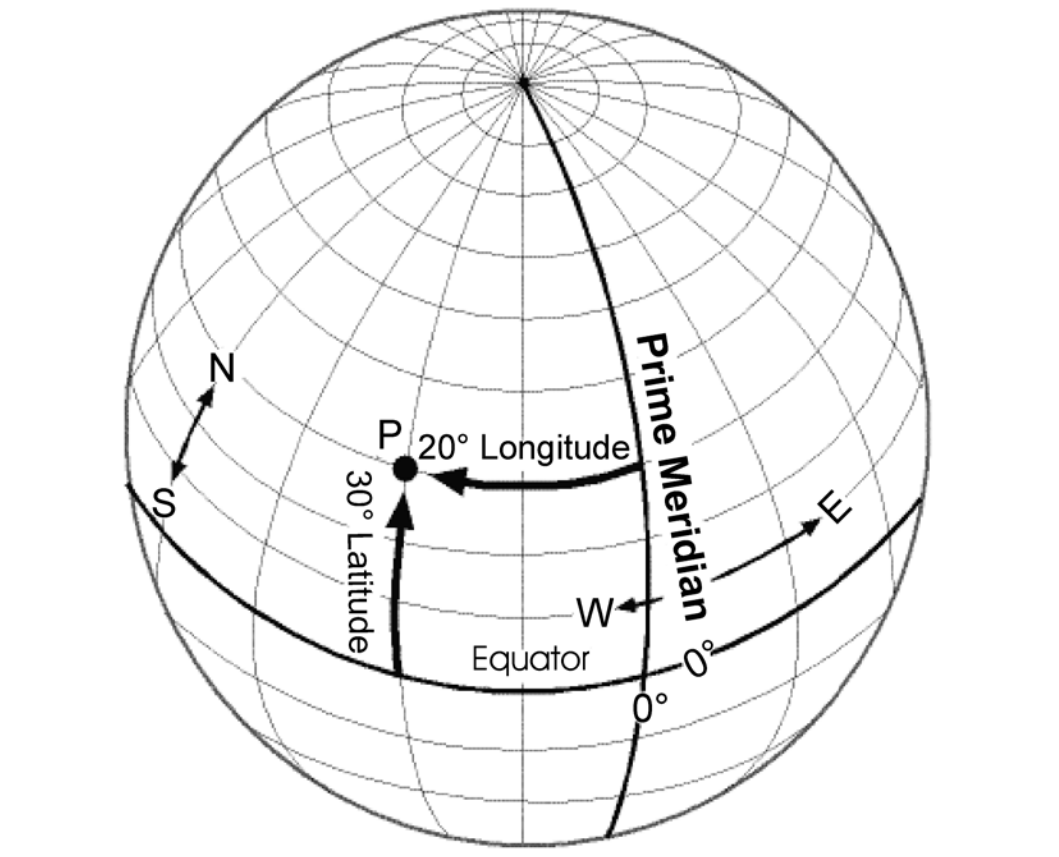
\includegraphics[width=10cm]{CoordenadasGeograficas.png}
    \caption{Representación de coordenadas geográficas. [Fuente: \citet{Fazal2008GISBasics}]}
    \label{fig:latitudLongitud}
\end{figure}

La elección arbitraria de una línea central de longitud corresponde a la que atraviesa el Observatorio Real en Greenwich, Inglaterra; se conoce como el meridiano de Greenwich o el meridiano principal, y las longitudes
al este u oeste se especifican como ángulos de giro con respecto al meridiano de Greenwich, variando de -180\grad (oeste) a 180\grad (este). La latitud es la distancia angular entre la línea ecuatorial (el ecuador), y un punto determinado de la Tierra, y las latitudes al sur y al norte varían en un rango de hasta 90\grad.

Las coordenadas geográficas son expresadas, por lo general, en grados, minutos y segundos, pero para su uso en los SIG son transformadas en grados decimales. Algunos ejemplos de las formas de representar las coordenadas ubicadas en un punto dentro de Asunción se muestran en la Tabla \ref{table:coordenadasGeograficas}.

\begin{table}[H]
\caption{Representación de coordenadas geográficas (WGS84).}
\centering
\begin{tabular}{cccc}
\hline
\multirow{2}{*}{Coordenadas} & \multirow{2}{*}{Grados, minutos y segundos} & \multicolumn{2}{c}{Grados decimales} \\ \cline{3-4} 
                             &                                             & Sin signo          & Con signo       \\ \hline
Latitud                      & 25\grad 16' 54.84'' Sur                            & 25.2819 Sur        & -25.2819        \\
Longitud                     & 57\grad 38' 6'' Oeste                                & 57.635 Oeste       & -57.635         \\ \hline
\end{tabular}
\label{table:coordenadasGeograficas}
\end{table}

\subsection{Sistema de coordenadas rectangulares}
Las proyecciones sirven para representar sobre un plano la superficie esférica de la Tierra con la menor deformación posible. El proceso de transferencia de la Tierra esférica a una superficie bidimensional, definidos normalmente mediante dos ejes perpendiculares \textit{XY} y en el caso de sistemas tridimensionales añadiendo un eje \textit{Z} perpendicular a ambos, introduce errores en los datos espaciales cuyo carácter variará dependiendo del método de proyección elegido. 

% Algunas proyecciones harán que la distancia entre las entidades espaciales se mantenga mientras la dirección está distorsionada. En otros casos, la forma puede conservarse a expensas de estimaciones de área precisas.

Podemos agruparlas en tres sistemas básicos según el tipo de plano auxiliar utilizado para proyectar la superficie terrestre: cilíndrica, cónica y acimutal (Ver Figura \ref{fig:capasGis}).

\begin{figure}[H]
    \centering
    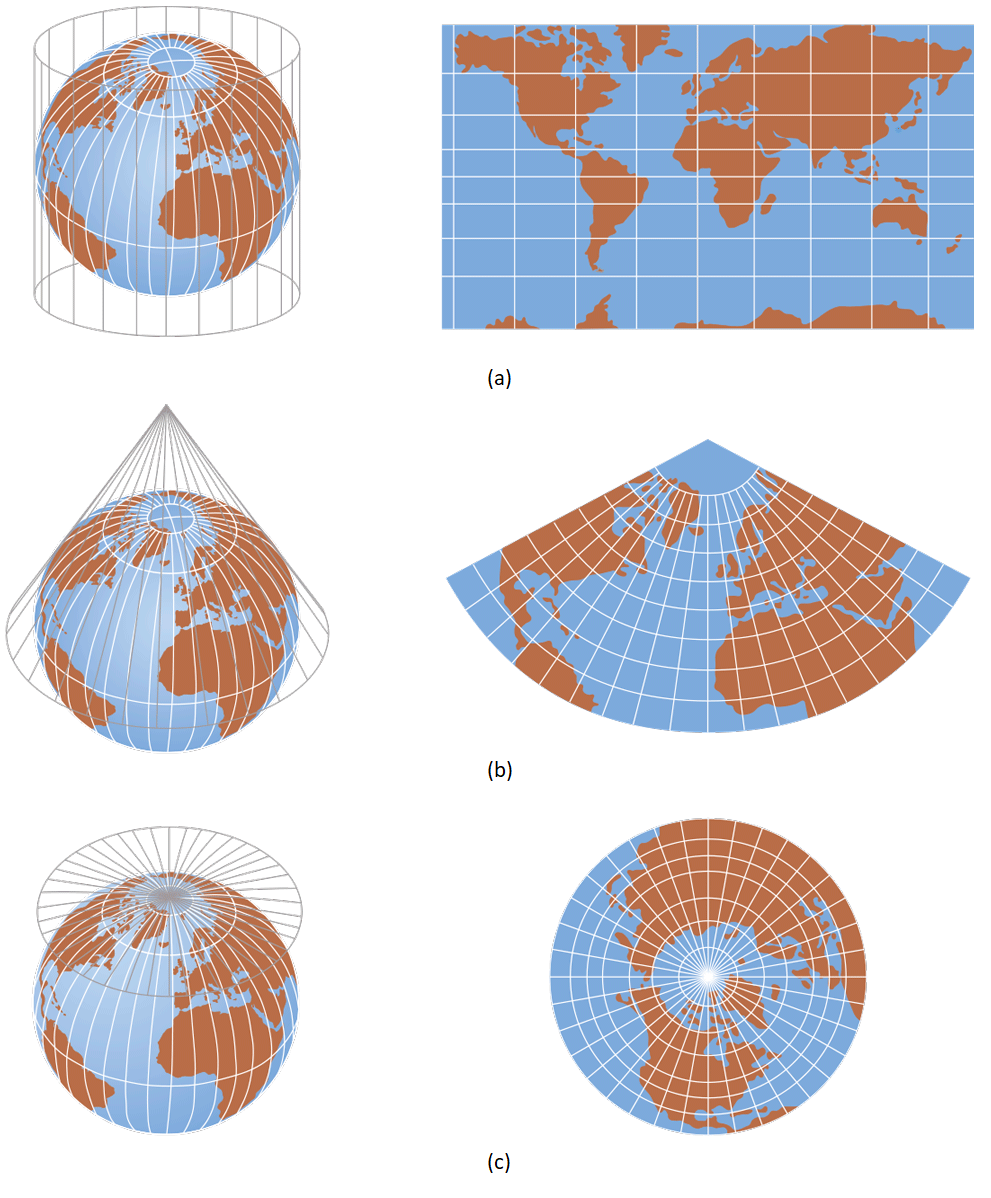
\includegraphics[width=10cm]{Chapter3/Chapter3Figs/CoordenadasProyectadas.png}
    \caption{Representación de tipos de proyecciones: (a) Cilíndrica (b) Cónica (c) Acimutal. [Fuente: blinklearning.com]}
    \label{fig:mapaCoordenadasGeograficas}
\end{figure}

Las proyecciones más sofisticadas permiten la preservación de representaciones precisas: de áreas, de distancias, de ángulos o de otras características; pero no todas ellas pueden conservarse en una misma proyección. De hecho, por lo general solo se puede mantener la  precisión de una sola característica y las demás se presentan distorsionadas con respecto a la realidad.

En Paraguay, cartógrafos y otros trabajadores en el área han adoptado el sistema de cuadrícula plana de \textit{Universal Transverse Mercator} (UTM), la cual corresponde a la proyección de tipo cilíndrica. Este sistema utiliza la proyección transversal de Mercator y divide la Tierra en 60 zonas verticales que tienen 6 grados de longitud, evitando los polos. El sistema se expresa en metros, facilitando así los cálculos de distancia y superficie.

En los SIG, los SRC están asociados a un identificador estándar único, denominados Identificador de Referencia Espacial (SRID, \textit{Spatial Reference System Identifier}), también son conocidos como códigos EPSG (\textit{European Petroleum Survey Group}) ya que existen varios SRID que han sido definidos por el EPSG. Como ejemplos tenemos el código EPSG 4326 que corresponde a WGS84 en coordenadas geográficas y el EPSG 32721 que es para la zona 21 Sur en coordenadas UTM, y así es como cada SRC tiene asociado un código único EPSG/SRID.

En la Tabla \ref{table:coordenadasPlanas} se muestran las coordenadas planas de la zona 21 Sur ó 21J de UTM/WGS84 que ubica un punto dentro de Asunción.

\begin{table}[H]
\caption{Representación de coordenadas planas (UTM).}
\centering
\begin{tabular}{cccc}
\hline
Coordenadas & UTM     & Zona & Hemisferio \\ \hline
X           & 436068  & 21 J & Sur        \\
Y           & 7203687 & 21 J & Sur        \\ \hline
\end{tabular}
\label{table:coordenadasPlanas}
\end{table}

\subsection{Sistema sin coordenadas}
Los sistemas sin coordenadas proporcionan referencias espaciales utilizando un código descriptivo en lugar de una coordenada. Los códigos postales ampliamente utilizados en todo el mundo son un ejemplo. Algunos códigos postales son totalmente numéricos, como los códigos postales estadounidenses, mientras que otros son alfanuméricos, como en el caso del código postal del Reino Unido.

Ejemplo de código postal en el Reino Unido: E1 6PX.

\section{Representación de los datos}

Las características de un mapa digital requieren ser representadas, y para ello se utilizan unas simbologías denominadas entidades espaciales cuyos tipos básicos son: puntos, líneas y áreas (Ver Figura \ref{fig:entidadesPuntoLineaPoligono}). Con estos tres tipos es posible de forma sencilla representar todos los fenómenos geográficos del mundo real a través de un mapa. Adicionalmente, hay otras entidades como las redes y superficies; que son extensiones de las líneas y áreas respectivamente.

\begin{figure}[H]
    \centering
    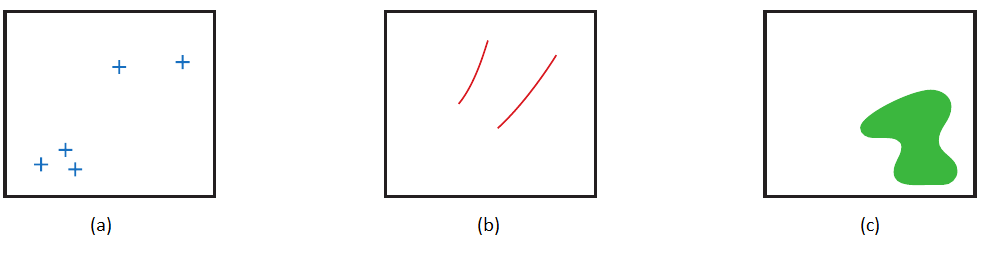
\includegraphics[width=10cm]{entidadesGeometricas.png}
    \caption{Entidades espaciales: (a) Puntos (b) Líneas (c) Áreas. [Fuente: \citet{Heywood2006AnSystems}]}
    \label{fig:entidadesPuntoLineaPoligono}
\end{figure}

Las características de un mapa a su vez pueden ser estructuradas mediante el uso de vectores y mediante el uso de matrices. Antes de detallar cada uno de estos sistemas, cabe mencionar que ambos se diferencian fundamentalmente en la estructura de los datos espaciales, en las relaciones topológicas, en el volumen físico de la información y en los métodos de análisis.

El concepto de Topología geoespacial es muy importante en los SIG y se lo define como ``el estudio de las relaciones espaciales entre las entidades espaciales y su posición en el mapa". Las relaciones topológicas, en relación a los datos, constan de tres elementos claves: adyacencia, contención y conectividad. En los sistemas matriciales las relaciones se producen entre celdas como análisis de vecindad generalmente; en los sistemas vectoriales se suelen basar en la relación arco-nodo que viene definida por la direccionalidad, la conectividad y la proximidad entre vectores.

\subsection{Sistema vectorial}

En el mundo vectorial, el punto es el bloque de construcción básico a partir del cual se construyen todas las entidades espaciales. El punto está representado por un único par de coordenadas (x,y). Las entidades de línea y área se construyen conectando una serie de puntos (Ver Figura \ref{fig:modeloVectorial}).

\begin{figure}[H]
    \centering
    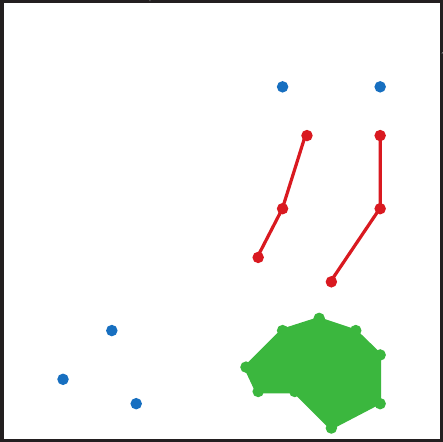
\includegraphics[width=7.5cm]{modeloVectorial.png}
    \caption{Representación de puntos, líneas y áreas en el sistema vectorial. [Fuente: \citet{Heywood2006AnSystems}]}
    \label{fig:modeloVectorial}
\end{figure}

Utilizando entidades de puntos se pueden representar cestos de basura residenciales, semáforos, árboles, alumbrados públicos. También a menor escala, es decir, en mapas más alejados y con menos detalle, puede utilizarse para indicar la ubicación de ciudades capitales. Las líneas se utilizan, mayormente, para representar calles, caminos, tendidos eléctricos, etc. Las áreas o polígonos corresponden a cuadras manzaneras, lotes, lagunas, países.

En el modelo vectorial, la representación de redes y superficies es una extensión del enfoque utilizado para almacenar entidades de línea y área respectivamente. Sin embargo, el método es más complejo y está estrechamente relacionado con la forma en que se estructuran los datos para la codificación por computadora.

Las líneas de contorno y las redes irregulares de triángulos (TIN; \textit{Triangulated Irregular Network}) se utilizan para representar la altitud u otros valores en continua evolución. Los TIN son registros de valores en un punto localizado, que están conectados por líneas para formar una malla irregular de triángulos. La cara de los triángulos representan, por ejemplo, la superficie del terreno.

\subsection{Sistema ráster}

En un sistema ráster, se ubica una cuadrícula imaginaria sobre el mapa. Cada celda de la cuadrícula, conocida como elemento de imagen o píxel, se examina para ver qué característica cae dentro de ella. El resultado final de este proceso es una cuadrícula o una serie de cuadrículas de números que representan las características en el mapa. (Ver Figura \ref{fig:modeloRaster}).

\begin{figure}[H]
    \centering
    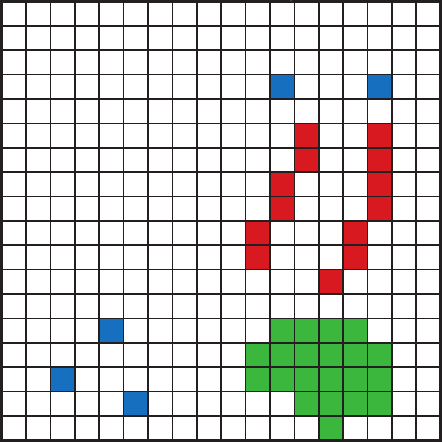
\includegraphics[width=7.5cm]{modeloRaster.png}
    \caption{Representación de puntos, líneas y áreas en el sistema ráster. [Fuente: \citet{Heywood2006AnSystems}]}
    \label{fig:modeloRaster}
\end{figure}

Este modelo se centra en las propiedades del espacio más que en la precisión de la localización. Divide el espacio en celdas regulares donde cada una de ellas representa un único valor. Se trata de un modelo de datos muy adecuado para la representación de variables continuas en el espacio. El tamaño de la celda de la cuadrícula es muy importante ya que influye en cómo aparece una entidad. En la Figura \ref{fig:rasterResolution} se muestra que cuanto mayores sean las dimensiones de las celdas menor es la precisión o detalle (resolución) de la representación del espacio geográfico.

\begin{figure}[H]
    \centering
    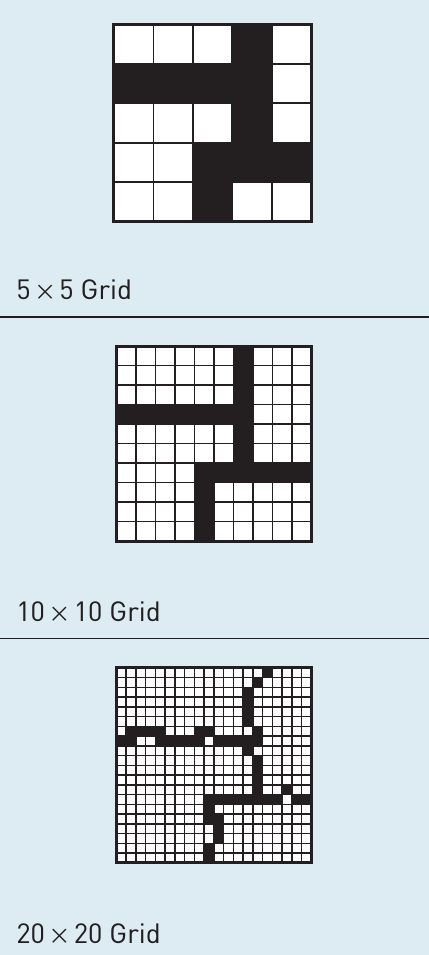
\includegraphics[width=6cm]{RasterResolution.png}
    \caption{Líneas con diferentes dimensiones de celdas. [Fuente: \citet{Heywood2006AnSystems}]}
    \label{fig:rasterResolution}
\end{figure}

% Hay varias variantes de la estructura de datos ráster de la cuadrícula regular, que incluyen: teselación irregular (por ejemplo, red irregular triangulada (TIN)), teselación jerárquica (por ejemplo, árbol cuádruple) y línea de escaneo \citep{Peuquet1991MethodsEnvironment}.

\section{Operaciones geométricas con datos vectoriales}

En esta sección veremos una serie de operaciones que transforman los datos vectoriales. Los resultados de algunas de estas operaciones son nuevas capas cuyas geometrías aportan información adicional a las geometrías originales, o bien las transforman para que su uso sea más adecuado en otros análisis u operaciones.

Existe una amplia gama de funciones para el análisis de datos disponibles en la mayoría de los paquetes SIG, que incluyen técnicas de medición, consultas de atributos, análisis de proximidad, operaciones de superposición y el análisis de modelos de superficies y redes \citep{Heywood2006AnSystems}. A continuación, se explican en qué consisten algunas de las técnicas sin profundizar en la complejidad de los algoritmos que son utilizados detrás de ellas.

\subsection{Medición}

El uso de las operaciones de medición es muy común en los SIG. En un vector, las distancias se miden utilizando el teorema de Pitágoras para obtener la distancia euclidiana. La geometría también se utiliza para calcular perímetros y áreas. Los perímetros se forman a partir de la suma de las longitudes de líneas rectas, y las áreas se calculan sumando las áreas de formas geométricas simples formadas por la subdivisión de la característica de interés \citep{Heywood2006AnSystems}.

Estas medidas, por lo general, son almacenadas como atributos de las entidades espaciales evitando así realizar el cálculo constantemente en cada consulta. Un detalle a tener en cuenta es que al almacenar estos atributos, cualquier modificación de geometría en la entidad debe ir seguida de la actualización de sus medidas de forma manual, de tal forma a mantener la consistencia en los datos.

\subsection{Zona de influencia}

La zona de influencia, conocida como \textit{buffering}, consiste básicamente en una región o polígono alrededor de una entidad. El término es relativamente simple, pero computacionalmente hablando resulta complejo. 

Para una entidad del tipo \textit{Point} su \textit{buffer} consiste en un círculo cuyo radio es la medida máxima de influencia definida. La creación de \textit{buffer} sobre los tipos \textit{Line} y \textit{Polygon} resultan conceptualmente similares, aunque los algoritmos subyacentes son notablemente más complejos (Ver Figuras \ref{fig:pointBuffer}, \ref{fig:lineBuffer} y \ref{fig:polygonBuffer}).

La distancia de \textit{buffer} puede ser variable conforme a valores numéricos incluidos en la tabla de atributos de la capa vectorial para cada entidad. Por ejemplo, con una capa de puntos que representen antenas de distintas potencias y alcances, pueden generarse zonas de influencia con radio distinto. En la Figura \ref{fig:lineBuffer}, se puede observar otro ejemplo donde la línea representa un río con el tamaño de \textit{buffer} definido en base a su caudal.

Los \textit{buffer} en torno a entidades poligonales se extienden normalmente hacia el exterior del borde del polígono aunque también es posible crear zonas de \textit{buffer} hacia el interior del borde del polígono.

\begin{figure}[H]
    \centering
    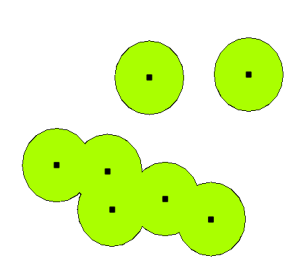
\includegraphics[width=4cm]{point_buffer.png}
    \caption{Representación de \textit{buffer} en puntos en el sistema vectorial. [Fuente: Documentación de QGis]}
    \label{fig:pointBuffer}
\end{figure}
% https://docs.qgis.org/2.14/es/docs/gentle_gis_introduction/vector_spatial_analysis_buffers.html

\begin{figure}[H]
    \centering
    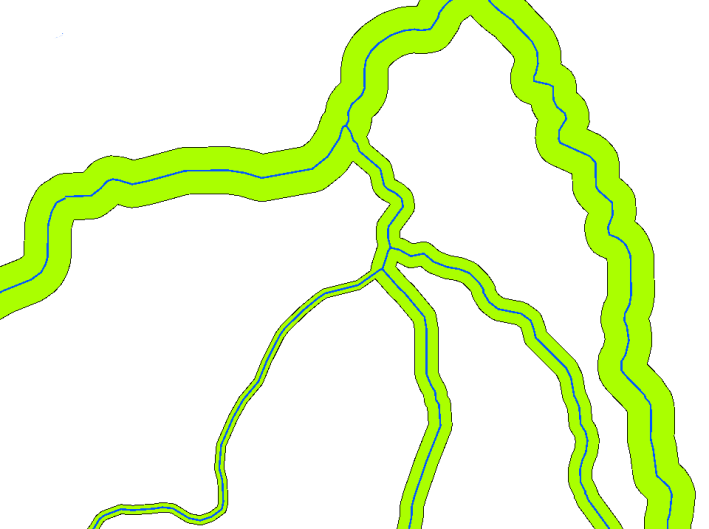
\includegraphics[width=4cm]{variable_line_buffer.png}
    \caption{Representación de \textit{buffer} variable en líneas en el sistema vectorial. [Fuente: Documentación de QGis]}
    \label{fig:lineBuffer}
\end{figure}

\begin{figure}[H]
    \centering
    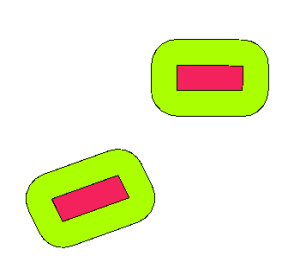
\includegraphics[width=4cm]{polygon_buffer.png}
    \caption{Representación de \textit{buffer} en áreas en el sistema vectorial. [Fuente: Documentación de QGis]}
    \label{fig:polygonBuffer}
\end{figure}

\subsection{Superposición}

Estas operaciones permiten generar nuevas capas vectoriales a partir de la fusión de datos de dos o más capas de datos de entrada, pudiendo dichas capas de origen contener distintos tipos de entidades. En los sistemas basados en vectores, la superposición de mapas requiere mucho tiempo, es compleja y computacionalmente costosa. En los sistemas basados en ráster, es justo lo contrario: rápido, directo y eficiente \citep{Heywood2006AnSystems}.

Ejemplos típicos de superposición espacial son:

\begin{itemize}
    \item Intersección: La capa de salida contiene todas las áreas donde ambas capas se solapan (intersectan).
    \item Unión: La capa de salida contiene todas las áreas de las dos capas de entrada combinadas.
    \item Diferencia simétrica: La capa de salida contiene todas las áreas de las capas de entrada excepto aquellas áreas en que ambas capas se solapan (intersección).
    \item Diferencia: La capa de salida contiene todas las áreas de la primera capa de entrada que no se solapan (intersectan) con la segunda capa de entrada.
\end{itemize} 
% \ref pagina de QGIS

\begin{figure}[H]
    \centering
    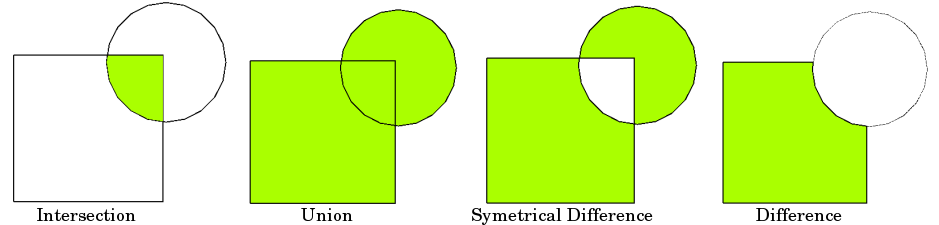
\includegraphics[width=8.5cm]{overlay_operations.png}
    \caption{La superposición espacial con dos capas de entrada vectoriales. La capa vectorial resultante se muestra en verde. [Fuente: Documentación de QGis]}
    \label{fig:overlay}
\end{figure}

\subsection{Disolución}

Esta operación recibe este nombre debido a que une polígonos con atributos comunes y disuelve las fronteras existentes entre ellos en una única entidad. No es necesario que exista una frontera entre los polígonos (es decir, que sean contiguos) ya que pueden almacenarse en una capa vectorial entidades compuestas por varios polígonos disjuntos. Esto se puede hacer con cualquier tipo de geometría: puntos, líneas o polígonos.
% \ref Víctor Olaya

\begin{figure}[H]
    \centering
    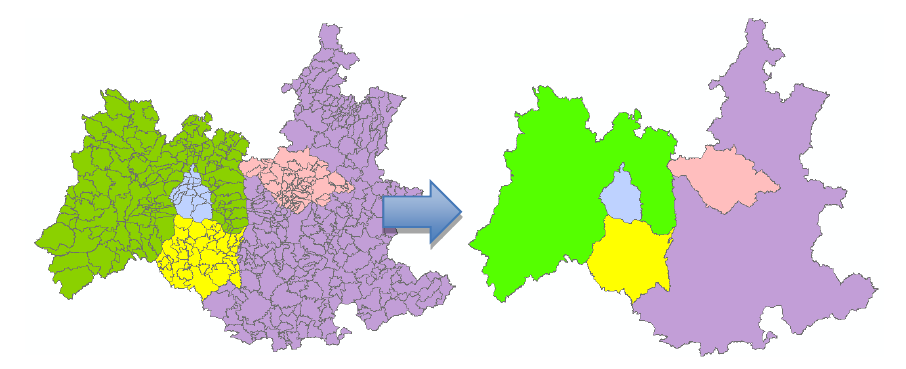
\includegraphics[width=8.5cm]{disolucion_vectorial.png}
    \caption{Operación de disolución o generalización. [Fuente: Algebra de Mapa. Diplomado]}
    \label{fig:disolution}
\end{figure}

\section{Almacenamiento espacial}

Una capa SIG puede ser almacenada con distintos formatos. Tanto para modelos del tipo vectorial como ráster existe un listado extenso de formatos que almacenan datos espaciales. Tal es así, que los software SIG han ido incorporando compatibilidad con los distintos formatos que iban surgiendo para no quedar relegados con otros de la competencia.

Los formatos de archivos SIG ráster mas tradicionales son: 
\begin{itemize}
    \item Esri Grid
    \item GeoTIFF
    \item JPEG 2000
    \item PNG
    \item MrSID
    \item ERDAS IMAGINE (IMG)
    \item ECW
    \item ASCII
    \item GeoPackage
    \item MBTiles
\end{itemize}

Por otro lado, entre los formatos SIG vectoriales más populares están: 
\begin{itemize}
    \item Esri shapefile
    \item CSV/GeoCSV
    \item DWG/DXF/DGN
    \item GML/XML
    \item GPX
    \item GeoPackage
    \item GeoJSON/TopoJSON
    \item GeoRSS
    \item KML/KMZ
    \item MapBox Vector Tiles (MVT)
\end{itemize}

Las capas también pueden ser almacenadas en base de datos relacionales y no relacionales, introduciendo el concepto de base de datos espaciales.

% Fuente:https://mappinggis.com/2015/12/los-formatos-gis-raster-mas-populares/

\subsection{Base de datos espaciales}

Las bases de datos espaciales se utilizan para almacenar datos espaciales. Por lo general, estas bases de datos agregan capacidades extras para manejar dicha información. Estas capacidades incluyen, por lo general, estructuración de datos espaciales, índices y funciones para la manipulación y análisis de la información.

El incremento del volumen de los datos ha derivado en la búsqueda de soluciones con alta escalabilidad en algunos \textit{software}. Se requiere que los \textit{software} tengan la capacidad de adaptarse y crecer en capacidad de trabajo o tamaño sin comprometer el rendimiento, funcionamiento y la calidad del mismo. Las bases de datos no han sido la excepción en esta búsqueda, y es así como el uso de las bases de datos conocidas como No-SQL se incrementó debido a las buenas prestaciones para el manejo de grandes volúmenes de datos (\textit{big data}) sobre las tradicionales conocidas como relacionales. Existen diferentes bases de datos No-SQL según su orientación: orientadas a documentos, a grafos, a columnas, entre otros.

Las bases de datos (BD) espaciales relacionales, sin embargo, siguen y seguirán siendo muy utilizadas por las ventajas que ofrecen sobre las demás en ciertos aspectos. A continuación, se mencionan características que difieren en ambas, pero que pueden variar con el paso del tiempo:

\begin{itemize}
    \item Las BD relacionales mantienen un formato único estructurado interno para almacenar la información geográfica, mientras que las No-SQL no lo tienen.
    \item Las BD No-SQL en ocasiones soportan algunas funcionalidades geométricas para gestionar datos geográficos sencillos. Las BD relacionales tienen una capacidad de análisis espacial mucho más sofisticada, funcionando como un auténtico SIG.
    \item Los SIG más utilizados para análisis espaciales complejos soportan conexiones con bases de datos relacionales, mientras que con No-SQL aún no son muy comunes dichos servicios.
\end{itemize}

Las bases de datos relacionales Postgres y Oracle agregan extensiones para soporte SIG que son PostGIS y Oracle Spatial and Graph, respectivamente. En el caso de PostGIS, al agregarse como extensión a una base de datos en Postgres, agrega un conjunto de funciones espaciales, tablas (donde almacenan las referencias espaciales SRID) y vistas (tablas lógicas que identifican las columnas geométricas de las diferentes tablas de la instancia de base de datos).

Actualmente existen estándares que definen este conjunto de tipos de datos y funciones espaciales mínimas para una base de datos SIG. El Open Geospatial Consortium (OGC) es un consorcio internacional de la industria cuyo objetivo es tratar de estandarizar la forma en que los datos geométricos y espaciales son accedidos y distribuidos. OGC cuenta con numerosas especificaciones que definen el acceso a los datos geoespaciales, servicios web para consulta y manipulación de datos, formatos de datos geoespaciales y consulta de datos geoespaciales.

\section{Mapas y Servidores de mapas}

Miles de páginas Web en internet incorporan mapas en sus sitios con diferentes fines. Estos sitios utilizan simplemente mapas del mundo preexistentes, es decir, no son mapas creados por el sitio, sino que en su mayoría utilizan servicios de mapas que están disponibles para incorporarlos en los diferentes \textit{software}.

Un mapa muy conocido es OpenStreetMap (también conocido como OSM), consiste en un proyecto colaborativo para crear mapas editables y libres. En lugar del mapa en sí, los datos generados por el proyecto se consideran su salida principal. Tanto las imágenes creadas como los datos vectoriales almacenados en su base de datos se distribuye bajo licencia abierta Licencia Abierta de Bases de Datos (ODbL; \textit{Open Database License}).

Otro proyecto de mapa del mundo con una larga trayectoria es Google Maps. Google Maps consiste en un servidor de aplicaciones de mapas en la web que pertenece a Alphabet Inc. Ofrece imágenes de mapas desplazables, así como fotografías por satélite del mundo e incluso la ruta entre diferentes ubicaciones, condiciones de tráfico en tiempo real y un calculador de rutas a pie, en coche, bicicleta y transporte público y un navegador GPS.

Proyectos como éstos ofrecen un listado de funcionalidades gratuitas y pagas. Algunas funcionalidades de ejemplo suelen ser obtener información del tráfico, camino más corto entre un punto de inicio y otro de llegada, ubicación de lugares por nombre, ubicación de calles, entre otros.

Del mismo modo, existen herramientas que permiten alojar nuestros propios mapas en un servidor y brindar servicios de mapa. Uno de ellos es GeoServer, el cual consiste en un servidor de código abierto escrito en Java que permite a los usuarios compartir y editar datos geoespaciales. Está diseñado para la interoperabilidad, publica datos de cualquier fuente de datos espaciales usando estándares abiertos. GeoServer es una implementación compatible con OGC de una serie de estándares abiertos, como el \textit{Web Feature Service} (WFS), el \textit{Web Map Service} (WMS), el \textit{Web Map Tile Service} (WMTS) y el \textit{Web Coverage Service} (WCS).